\documentclass{article}
\usepackage{graphicx}
\usepackage[utf8]{inputenc}
\usepackage{listings}
\usepackage{color}
\usepackage{xcolor}
\usepackage{textcomp}
\usepackage{amsmath}
\begin{document}

\title{Tarea Newton no Lineal}
\author{Angel Caceres Licona}

\maketitle


\section{Aproxime la solución de los siguientes sistemas usando el método de Newton\dots}
\subsection{Primer inciso}
Tenemos la siguiente gráfica:
\begin{center}
    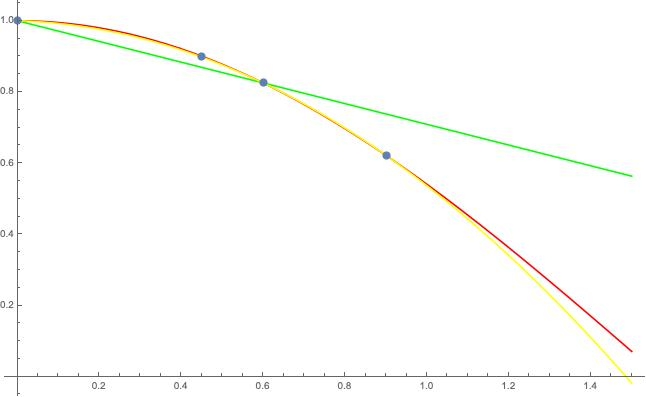
\includegraphics[scale=0.5]{Grafica1.png}    
\end{center}
Por lo que vemos que tiene una raiz aproximadamente en $(-0.1, -0.2)$.\\ 
Corremos el programa y obtenemos: $(0.121242,0.271105)$ después de 5 iteraciones.\\
Para la segunda raíz escogemos $(0.1, 0.3)$ y obtenemos $( 0.121242,0.271105)$ después de 7 iteraciones.

\subsection{Segundo inciso}
Tenemos la siguiente gráfica:
\begin{center}
    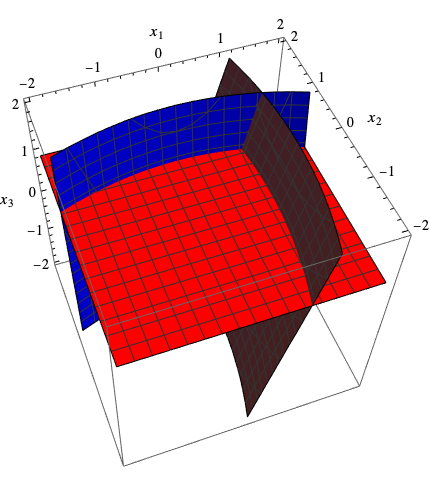
\includegraphics[scale=0.5]{grafica2.png}    
\end{center}
Por lo que vemos que tiene una raiz aproximadamente en $(1, 1, 1)$.\\
Corremos el programa y obtenemos: ${1.03177,1.08488,0.91337}$

\subsection{Tercer inciso}
Tenemos la siguiente gráfica:
\begin{center}
    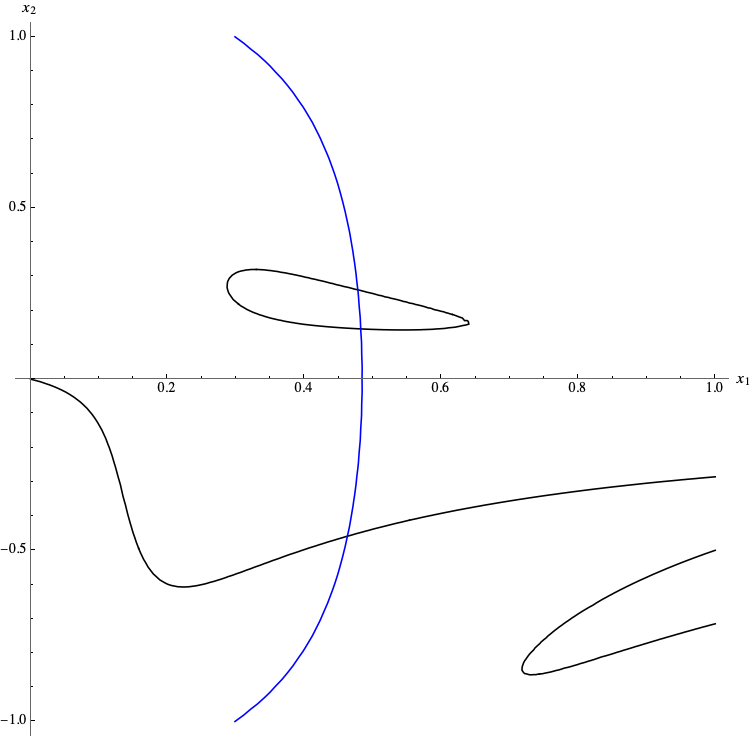
\includegraphics[scale=0.5]{grafica3.png}    
\end{center}
Por lo que vemos que tiene una raiz aproximadamente en $(0.5, -0.5)$.\\
Corremos el programa y obtenemos: ${0.463042,-0.458809}$\\
Vemos que hay otra raiz aproximadamente en ${0.5,0.1}$\\
Corremos el programa y obtenemos: ${0.48257,0.14623}$\\
Vemos que hay otra raiz aproximadamente en ${0.5,0.3}$\\
Corremos el programa y obtenemos: ${0.478155,0.26092}$\\

\end{document}